\documentclass[conference]{IEEEtran}

% ---- packages ----
\usepackage[T1]{fontenc}
\usepackage{amsmath,amssymb}
\usepackage{graphicx}
\usepackage{xcolor}
\usepackage{subfig}        % \subfloat
\usepackage{pgfplots}
\pgfplotsset{compat=1.18}

% ---- spacing (控えめに詰める) ----
\setlength{\textfloatsep}{8pt plus 2pt minus 2pt}
\setlength{\intextsep}{6pt plus 2pt minus 2pt}
\setlength{\abovecaptionskip}{4pt}
\setlength{\belowcaptionskip}{4pt}

% ---- figure sizes ----
\newlength{\figW}\setlength{\figW}{0.95\columnwidth}
\newlength{\figH}\setlength{\figH}{0.60\columnwidth}   % 基準
\newlength{\figHbig}\setlength{\figHbig}{0.90\columnwidth} % 縦1.5倍相当

% ---- pgfplots 共通スタイル ----
\pgfplotsset{
  myaxis/.style={
    width=\figW,height=\figH,
    grid=both, grid style={line width=.1pt, draw=gray!30},
    major grid style={line width=.2pt, draw=gray!60},
    tick align=outside,
    legend cell align=left
  },
  myaxisbig/.style={
    width=\figW,height=\figHbig,
    grid=both, grid style={line width=.1pt, draw=gray!30},
    major grid style={line width=.2pt, draw=gray!60},
    tick align=outside,
    legend cell align=left
  }
}

\begin{document}
\title{SystemDK with AITL: (Draft)}
\author{Anonymous}
\maketitle

\begin{abstract}
This paper introduces SystemDK with AITL ...
\end{abstract}

\section{Introduction}
本文……(略)

%==================== Fig.1 ====================
\begin{figure}[t]
  \centering
  % Fig.1 はみ出し防止 (幅は列幅の95%)、clipで余白カットしても絵は欄内
  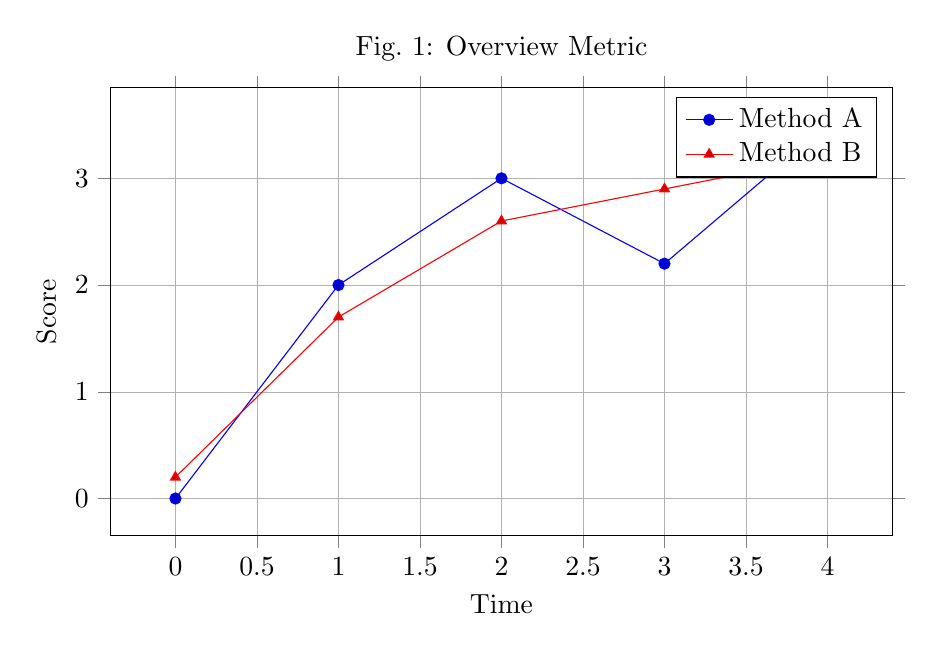
\begin{tikzpicture}
    \begin{axis}[
      myaxis,
      xlabel={Time}, ylabel={Score},
      title={Fig.~1: Overview Metric},
      clip mode=individual
    ]
      \addplot+[mark=*] coordinates {(0,0) (1,2) (2,3) (3,2.2) (4,3.5)};
      \addplot+[mark=triangle*] coordinates {(0,0.2) (1,1.7) (2,2.6) (3,2.9) (4,3.2)};
      \legend{Method A, Method B}
    \end{axis}
  \end{tikzpicture}
  \caption{System-level overview plot (column-safe width).}
  \label{fig:fig1}
\end{figure}

\section{Approach}
本文……(略)

%==================== Fig.2: (a)(b)(c) 縦並び・間隔広め ====================
\begin{figure}[t]
  \centering
  % ---- (a) ----
  \subfloat[(a) Throughput vs. Load]{%
    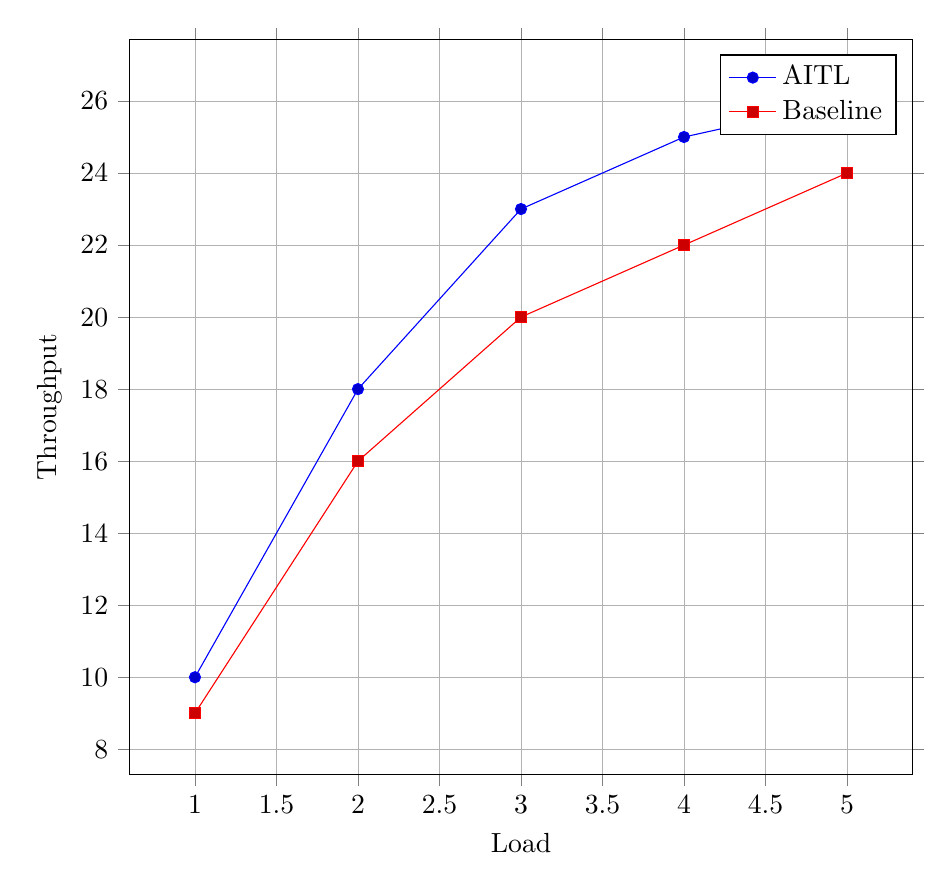
\begin{tikzpicture}
      \begin{axis}[
        myaxisbig,
        xlabel={Load}, ylabel={Throughput}
      ]
        \addplot+[mark=*] coordinates {(1,10) (2,18) (3,23) (4,25) (5,26)};
        \addplot+[mark=square*] coordinates {(1,9) (2,16) (3,20) (4,22) (5,24)};
        \legend{AITL, Baseline}
      \end{axis}
    \end{tikzpicture}
  }\\[8pt]
  % ---- (b) 凡例はグラフ外 (south outside) で重なり回避 ----
  \subfloat[(b) Latency distribution]{%
    \begin{tikzpicture}
      \begin{axis}[
        myaxisbig,
        xlabel={Percentile}, ylabel={Latency (ms)},
        legend pos=south outside
      ]
        \addplot+[mark=none] coordinates {(50,12) (75,15) (90,18) (95,22) (99,35)};
        \addplot+[mark=none, dashed] coordinates {(50,14) (75,18) (90,24) (95,30) (99,48)};
        \legend{AITL, Baseline}
      \end{axis}
    \end{tikzpicture}
  }\\[8pt]
  % ---- (c) ----
  \subfloat[(c) Resource heat map (toy)]{%
    \begin{tikzpicture}
      \begin{axis}[
        myaxisbig,
        view={0}{90}, % 2D heatmap風
        xlabel={Core}, ylabel={Task},
        colormap name=viridis,
        colorbar, colorbar style={title=util}
      ]
        % 小さなおもちゃデータ(そのままコンパイル可)
        \addplot[matrix plot*, point meta=explicit] coordinates {
          (1,1) [1]  (2,1) [2]  (3,1) [3]  (4,1) [2]
          (1,2) [2]  (2,2) [3]  (3,2) [4]  (4,2) [3]
          (1,3) [1]  (2,3) [2]  (3,3) [2]  (4,3) [1]
        };
      \end{axis}
    \end{tikzpicture}
  }

  \caption{Fig.~2: (a)--(c) are vertically stacked with wider spacing; (b) legend is placed outside to avoid overlap.}
  \label{fig:fig2}
\end{figure}

\section{Evaluation}
本文……(略)

\section{Conclusion}
本文……(略)

% 参考文献のバランス調整(必要に応じて番号を変更)
\IEEEtriggeratref{4}

\begin{thebibliography}{00}
\bibitem{r1} A. Author, “Title,” Venue, Year.
\bibitem{r2} B. Author, “Title,” Venue, Year.
\bibitem{r3} C. Author, “Title,” Venue, Year.
\bibitem{r4} D. Author, “Title,” Venue, Year.
\bibitem{r5} E. Author, “Title,” Venue, Year.
\end{thebibliography}

% IEEEtran の conference モードは \IEEEbiography がロックされるため、
% セクション素の体裁で代替します(2ページ右欄に寄せたい場合は
% \IEEEtriggeratref の位置や数で微調整)。
\section*{Author Biography}
\small
Shinichi T., received the B.E. ... (略)。Contact: \texttt{shin3t72@gmail.com}

\end{document}
